\documentclass{article}
\usepackage[utf8]{inputenc}
\usepackage{polski}
\usepackage[lined,boxed]{algorithm2e}
\usepackage{float}
\usepackage{graphicx}
\title{Sprawozdanie}
\author{Kajetan Bilski 244942}

\begin{document}
	\maketitle
	\pagenumbering{arabic}

\section{Opis programu}
Cały program jest w pliku blocksys.jl, który zawiera tylko moduł blocksys, w którym są wszystkie funkcje programu. Wszystkie liczby rzeczywiste są zapisywane jako Float64.
\subsection{loadMatrix(filename)}
Funkcja zwraca trójkę \verb|(A,n,l)|, gdzie \verb|A| to macierz załadowana z pliku o nazwie \verb|filename| jako \verb|SparseArray|.
\subsection{loadVector(filename)}
Funkcja zwraca wektor \verb|b| z pliku o nazwie \verb|filename|.
\subsection{generateB(A,n,l)}
Funkcja mnoży macierz \verb|A| przez wektor jedynek o długości \verb|n| i zwraca wynik \verb|b|. Przy mnożeniu dla każdego wiersza funkcja bierze pod uwagę tylko pola, które według zadanej postaci macierzy $A$ są niezerowe. Dla stałego $l$ daje to złożoność $O(n)$.
\subsection{elimination(A,b,n,l,withChoice)}
Funkcja dokonuje eliminacji Gaussa w celu znalezienia rozwiązania $Ax=b$ i zwraca wektor \verb|x|. Żeby nie zmieniać \verb|A| ani \verb|b| poza funkcją, najpierw robiona jest głęboka kopia obu zmiennych.\\
Jeżeli \verb|n == l|, to znaczy, że macierz jest gęsta i funkcja wykonuje standardową wersję eliminacji Gaussa zmieniając przy tym postać \verb|A| i \verb|b|. Najpierw w \verb|n| krokach macierz \verb|A| zamieniana jest na macierz trójkątną. W każdym kroku $i = 1,2,...,n$ dla każdego wiersza $j > i$ liczone jest $l_{i j} = \verb|A[i,j] / A[i,i]|$, następnie dla każdego $x \geq i$, $\verb|A[x,j]| = \verb|A[x,j]| - \verb|A[x,i]| * l_{i j}$ i na końcu $\verb|b[j]| = \verb|b[j]| - \verb|b[i]|$. Otrzymujemy macierz $U$. Ta część funkcji składa się z 3 zagnieżdżonych pętli o złożoności $O(n^3)$. Po przekształceniu \verb|A| i \verb|b| funkcja oblicza wektor $\verb|x[1]|,\verb|x[2]|,...,\verb|x[n]|$. W pętli dla $i$ malejącego od \verb|n| do $1$ obliczane jest $\verb|x[i]| = \frac{b[i] - A[n,i] * x[n] - A[n-1,i] * x[n-1] - ... - A[i+1,i] * x[i+1]}{A[i,i]}$. Ta część funkcji przechodzi raz po każdym niezerowym polu macierzy trójkątnej co daje złożoność $O(n^2)$. Wektor \verb|x| jest rozwiązaniem \verb|Ax=b|. Jeżeli \verb|withChoice| jest prawdą to funkcja działa w trybie z częściowym wyborem elementu głównego. Wtedy przed każdym krokiem $i = 1,...,n$ eliminacji szukany jest wiersz o numerze $y = i,i+1,...,n$ z największym $i$-tym elementem, wybrany wiersz zostaje zamieniony miejscami z $i$-tym. Żeby sama zamiana zachowała złożoność $O(1)$ wartości w macierzy nie są zmieniane, zamieniane są tylko numery wierszy w osobnej tablicy referencji pamiętającej miejsce przechowywania każdego wiersza. Złożoność operacji wyboru elementu głównego ma złożoność $O(n)$, ale wykonuje się ona zawsze przed pętlą, której złożoność wynosi $O(n^2)$, więc wybór nie ma wpływu na ogólną złożoność. Złożoność całej funkcji w tym przypadku jest równa $O(n^3)$, ale \verb|n| jest równe \verb|l|, które jest stałą, więc $O(n^3) = O(l^3) = O(1)$.\\
Jeżeli $\verb|n| > \verb|l|$ to znaczy że macierz nie jest gęsta i funkcja stosuje usprawnienia dla pomijania działań na zerach. Macierz \verb|A| podzielona jest na "bloki" gdzie w każdym bloku wszystkie wiersze mają swoje piersze (od lewej) niezerowe pola w tej samej kolumnie $x$ i same zerowe pola od kolumny $x+2l+2$. W każdym $i$-tym kroku zamiast mnożyć i odejmować cały $i$-ty wiersz od wszystkich o numerach $>i$, modyfikowane są tylko wiersze i kolumny do końca bloku. Jeśli $i$ jest większe lub równe indeksowi kolumny w której znajdują się pierwsze pola niezerowe następnego bloku, to modyfikowane się wiersze i kolumny do końca następnego bloku. Tak samo zmniejszony jest zakres wyboru elementu głównego. Zmniejsza to złożoność tej części funkcji do $O(n*l^2)$. W drugiej części do obliczania każdego \verb|x[i]| też wykorzystywane jest to, że w każdym wierszu wszystkie pola niezerowe w $i$-tym wierszu mieszczą się w kolumnach od $i$ do $i+2l+1$, co zmniejsza złożoność do $O(n*l)$. W tym przypadku złożoność całej funkcji wynosi $O(n*l^2)=O(n)$.
\subsection{decomposition(A,n,l,withChoice)}
Funkcja dokonuje rozkładu LU macierzy \verb|A| z opcjonalnym częściowym wyborem elementu głównego i zwraca trójkę \verb|(LU,ref,nzCount)|, gdzie \verb|ref| jest wektorem pamiętającym indeksy wierszy, a \verb|nzCount| jest wektorem wektorów pamiętającym położenie pól niezerowych w macierzy $L$. Funkcja najpierw robi głęboką kopię \verb|A|, żeby nie zmieniać jej poza sobą.\\
Działa ona podobnie jak pierwsza część funkcji \verb|elimination| z tą różnicą że w \verb|elimination| zapisywana była tylko macierz $U$ podczas gdy tutaj trzeba pamiętać też $L$ oraz nie używany jest wektor \verb|b|. Macierz $LU$ zapisywana jest w sposób pokazany na wykładzie w miejscu macierzy \verb|A|.\\
Po obliczeniu każdego $l_{i j} = \verb|A[i,j]| / \verb|A[i,i]$ podstawiane jest $\verb|A[i,j]|=l_{i j}$. Oprócz tego do pamiętania niezerowych wartości używany jest wektor wektorów \verb|nzCount|, gdzie \verb|nzCount[i]| jest wektorem kolumn w których znajdują się wszystkie niezerowe pola $i$-tego wiersza macierzy $L$ (nie licząc pól na przekątnej). Do \verb|nzCount| na bierząco w czasie $O(1)$ dopisywane są numery pól jak są wstawiane. W każdej kolumnie $L$ jest co najwyżej $l+2$ pól niezerowych, czyli $O(n*l)$, co będzie ważne dla funkcji \verb|solveWithLU|. Złożoność jest taka sama jak \verb|elimination|, czyli $O(n)$.
\subsection{solveWithLU(LU,ref,nzCount,n,l,b)}
Funkcja rozwiązuje równanie $LUx=b$ i zwraca \verb|x|.\\
Funkcja rozwiązuje dwa trójkątne układy równań $Ly=b$ i $Ux=y$, w tej kolejności. Żeby obliczyć $y$, używany jest wzór dla $i = 1,2,...,n$, $y_i = \verb|b[i]| - \verb|A[1,i]| * y_1 - \verb|A[2,i]| * y_2 - ... - \verb|A[i-1,i]| * y_{i-1}$. Używamy tylko niezerowych wartości z \verb|A|, które znamy z \verb|nzCount| i wiedząc że jest ich $O(n*l)$, otrzymujemy taką samą złożoność. W drugiej części funkcja oblicza $Ux=y$ w taki sam sposób jak w \verb|elimination| w czasie $O(n*l)$. Złożoność całej funkcji wynosi $O(n*l)=O(n)$.
\subsection{getError(x,n)}
Funkcja zwraca błąd względny obliczany wzorem \verb|norm(x - ones(n)) / norm(ones(n))|.
\subsection{printX(filename,x,n,withError)}
Funkcja zapisuje do pliku o \verb|filename| wektor \verb|x|. Jeżeli \verb|withError| jest prawdą to w pierwszej linijce zapisuje błąd względny zwrócony przez \verb|getError()|.
\section{Eksperymenty}
\begin{figure}[H]
	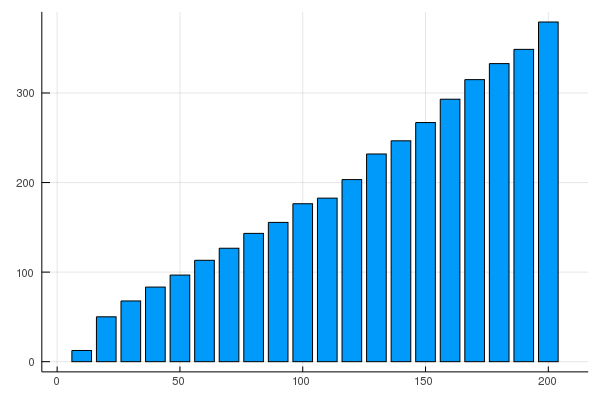
\includegraphics[width=\linewidth]{n_elimination_noChoice.png}
	\caption{Czas rozwiązywania $Ax=b$ metodą eliminacji Gaussa w milisekundach w zależności od $n$.}
	\label{fig:asdf}
\end{figure}
\begin{figure}[H]
	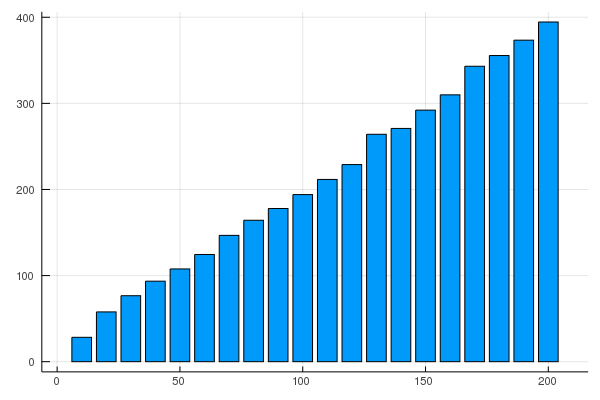
\includegraphics[width=\linewidth]{n_withLU_noChoice.png}
	\caption{Czas rozwiązywania $Ax=b$ dwuetapowo z rozkładem LU w milisekundach w zależności od $n$.}
	\label{fig:asdf}
\end{figure}
Jak widać z wykresów złożoność czasowa obu algorytmów w zależności od $n$ jest liniowa.\\
\begin{figure}[H]
	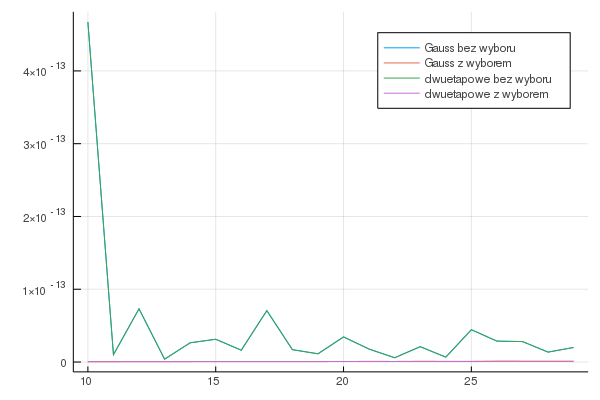
\includegraphics[width=\linewidth]{precision_cond.png}
	\caption{Błąd względny wyniku w zależności od współczynnika uwarunkowania macierzy $A$.}
	\label{fig:asdf}
\end{figure}
\begin{figure}[H]
	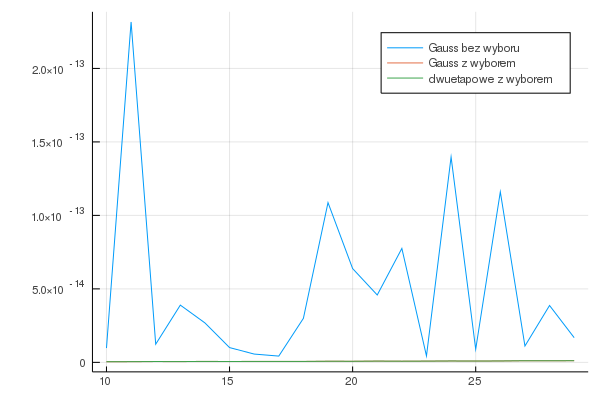
\includegraphics[width=\linewidth]{precision_cond_2.png}
	\caption{Błąd względny wyniku w zależności od współczynnika uwarunkowania macierzy $A$.}
	\label{fig:asdf}
\end{figure}
\begin{figure}[H]
	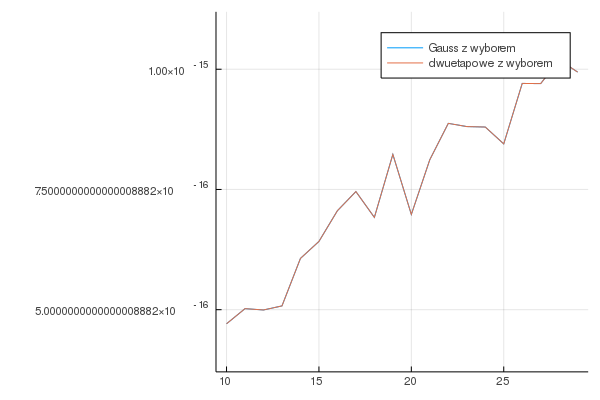
\includegraphics[width=\linewidth]{precision_cond_3.png}
	\caption{Błąd względny wyniku w zależności od współczynnika uwarunkowania macierzy $A$.}
	\label{fig:asdf}
\end{figure}
Jak widać największe błędy generuje metoda dwuetapowa bez wyboru elementu głównego, potem metoda eliminacji Gaussa bez wybory, a obie metody z częściowym wyborem dają takie same błędy względne.\\
\begin{figure}[H]
	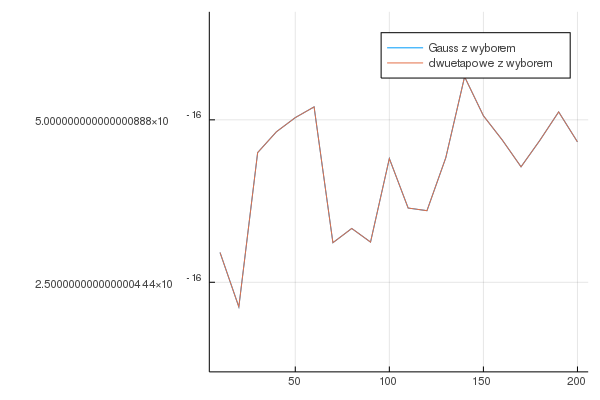
\includegraphics[width=\linewidth]{precision_n_3.png}
	\caption{Błąd względny wyniku w zależności od współczynnika uwarunkowania macierzy $A$.}
	\label{fig:asdf}
\end{figure}
Błąd względny jest rośnie wraz ze wzrostem $n$ lub współczynnika uwarunkowania macierzy.
\end{document}